\documentclass[11 pt]{scrartcl}
\usepackage[header, margin, koma, stylish]{chen}
\usepackage{csquotes}
\usepackage{caption}
\usepackage{todonotes}

\pagestyle{fancy}
\fancyhf{}
\fancyhead[l]{CS 161 Notes}
\fancyhead[r]{Chufan Chen}
\cfoot{\thepage}

\newcommand{\tx}{\tilde{x}}
\newcommand{\eq}{\text{eq}}
\newcommand{\opt}{\text{opt}}
\newcommand{\nz}{\text{nz}\,}
\newcommand{\epi}{\text{epi}\;}

\begin{document} 
\title{\Large CS 161: Computer Security}
\author{\large Chufan Chen}
\date{\large\today}

\maketitle 

\begin{center}
\begin{displayquote}
    \emph{"A good stock of examples, as large as possible, is indispensable for a thorough understanding of any concept, and when I want to learn something new, I make it my first job to build one."} \\ \begin{flushright} \emph{– Paul Halmos}.  \end{flushright}
\end{displayquote}
\begin{displayquote}
    \emph{"Constrained optimization is the art of compromise between conflicting objectives."} \\ \begin{flushright} \emph{– William A. Dembski}.  \end{flushright}
\end{displayquote}
\end{center}


\tableofcontents 

\newpage

\section{Wednesday, August 25th: Introduction}
\subsection{Course Outline}
\itemnum
    \ii Introduction to Security
    \ii Memory Safety
    \ii Cryptography
    \ii Web Security
    \ii Network Security
    \ii Miscellaneous Topics
\itemend

\subsection{What is Security}
Security enforcing a desired property in the presence of an attacker. These property includes:
\itemnum
    \ii data confidentiality
    \ii user privacy
    \ii data and computation integrity
    \ii authentication
    \ii avaliablity
\itemend
Security is important for our
\itemnum
    \ii physical safety
    \ii confidentiality/privacy
    \ii functionality
    \ii protecting our assets
    \ii successful business
    \ii a country’s economy and safety
\itemend
Everthing is hackable, especially things connected to the Internet.\newline
What will you learn in this class?
\itemnum
    \ii How to think adversarially about computer systems
    \ii How to assess threats for their significance
    \ii How to build programs \& systems with robust security properties
    \ii How to gauge the protections and limitations provided by today's technology
    \ii How attacks work in practice
\itemend
The rest of this lecture is largely focused on philosophical issues.
\itemnum
    \ii People and Money
    \ii Threat Model
\itemend
\subsection{People and Money}
People attack systems for some reason. Often the most effective security is to attack the attacker's motivation.\newline
It All Comes Down to People... \newline
The Attackers\newline
People attack systems for some reason\newline
No attackers? No problem!
\itemnum
    \ii They may do it for money
    \ii They may do it for politics
    \ii They may do it for the lulz
    \ii They may just want to watch the world burn
\itemend
\subsection{Threat Model}
For personal security, it best described by threat model and chill.\newline
Threat Model is about who and why might someone attack you? 
\itemnum
    \ii Criminals for money
    \ii Teenagers for laughs or to win in an online game
    \ii Governments
    \ii Intimate partners threat
\itemend
We talked a lot about threat model because when you think about secuity you shouldn't just ask yourself this binary question is it secure or not but secuity  against who, secure against what, what types of attackers, who might be
trying to attack your system, what might their motivation be, what might their
resources and their capabilities be, and we often don't need to defend against everyone maybe there's just some subset of people we need to defend against.
Often the most effective security is to attack the reasons for an attacker.\newline
It All Comes Down to People... \newline
The Users\newline
Have you ever sacrificed your own personal security for the sake of usability?
\itemnum
    \ii If a security system is unusable it will be unused
    \ii Users will subvert systems anyway
    \ii Programmers will make mistakes
    \ii Social Engineering
\itemend
But don't blame the Users
\itemnum
    \ii Often we blame the user when an attacker takes advantage of them.
    \ii Phishing is a classic example
\itemend
Security often comes down comes down to money 
\itemnum
    \ii "You don't put a \$10 lock on a \$1 rock Unless the attacker can leverage that \$1 rock to attack something more important
    \ii "You don't risk exposing a \$1M zero-day on a nobody"
    \ii Cost/benefit analyses appear all throughout security
\itemend
\textbf{Prevention}\newline
The goal of prevention is to stop the "bad thing" from happening at all. On one hand, if prevention works its great. E.g. if you don't write in an unsafe language (like C) you will never worry about buffer overflow exploits. On the other hand, if you can only depend on prevention. You get Bitcoin and Bitcoin thefts.\newline
\textbf{Detection and Response}\newline
Detection: See that something is going wrong\newline
Response: Actually do something about it\newline
False Positive and False Negatives\newline
False positive: You alert when there is nothing there \newline
False negative: You fail to alert when something is there \newline
This is the real cost of detection:\newline
Responding to false positives is not free. And too many false positives and alarms get removed.False negatives mean a failure.\newline
\textbf{Defense in Depth}\newline
The notion of layering multiple types of protection together. Hypothesis is that attackers needs to breech all the defenses. But defense in depth isn't free. You are throwing more resources at the problem. You can have a incresead false positive rate.\newline
\textbf{Mitigation and Recovery}
The bad things happened, can we get back on our feet. Assumption: bad things will happen in the system, so can we design things so we can get back working? Back it up!\newline
\textbf{Password}\newline
Humans can't remember good passwords.\newline
\begin{figure}[!htb]
    \centering
    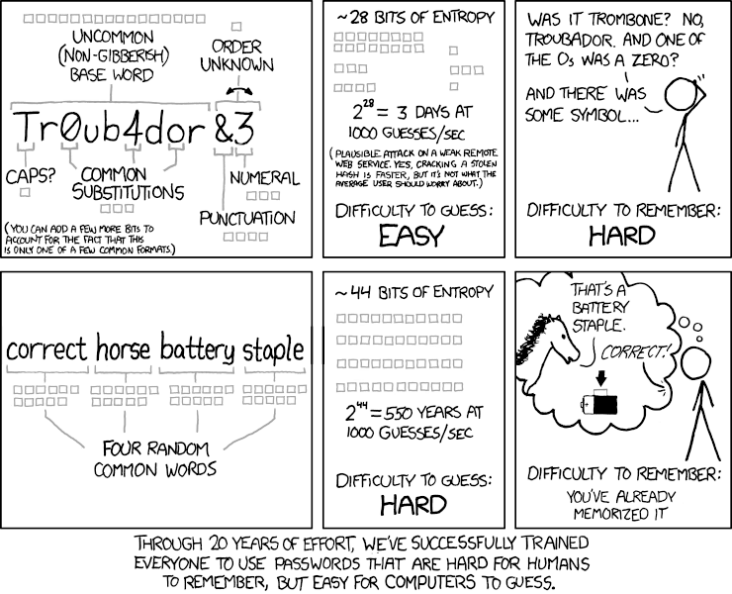
\includegraphics[scale=0.5]{assets/password.png}
    \caption{Password.}
\end{figure}
Something you know. Password\newline
Something you have. RSA token\newline
Something you are. Fingerprint\newline
So what to do? Password Managers! E.g. 1Password\newline
And FIDO U2F Security Keys is a very powerful second-factor for 2-factor authentication. This can not be phished.
\newpage
\section{Thursday, November 4th: Security Principles}
\subsection{The Properties We Want in a Safe}
We want the inside to be inaccessible to an attacker. But what \textbf{sort} of attacker? And \textbf{how much time does} the attacker have? We want to measure how much time \& capabilities needed for an attacker. For a safe, ratings communicate how much based on experts performing the attack. Such secuirty ratings are much harder in the computer security side.
\begin{example}
    Security Rating: A Real Safe\newline
    TL-15(\$3,000): An expert with common tools will take $\ge 15$ minutes to break in. May even have "relockers".\newline
    TLRTL-30(\$10,000): 30 minutes with common tools and a cutting torch.\newline
    Gun Safe: Meets the California requirements for safe storage of a handgun. But it is practically snake oil. It create an iluusion of security. It meets the legal requirement for security.
\end{example}
Lesson from safe: Security is economics. More security costs more. Standards often define security.\newline
We've seen that laptop/desktop platforms grant application a lot of privilege. \newline
\textbf{Thinking About Least Privilege}\newline When assessing the security of a system's design, identify the Trusted Computing Base(TCB). What components deos secuirty rely upon? Security requires that the TCB: correct, comlete(can't be bypassed) and secure(can't be tampered with). Best way to be assured of correctness and its security are KISS(Keep It Simple, Stupid) and Generally, Simple(Small). One powerfuldesign approach: privilege separation. Isolate privileged operations to as small a component as possible.
\textbf{The Base for Isolation: The Operating Systems}\newline
The operating systems process provide the following "guarentees".
\itemnum
    \ii Isolation: A process can not access(read or write) the memory of any other process.
    \ii Premissions: A process can only change files etc if it has permission to 
\itemend
\begin{figure}[!htb]
    \centering
    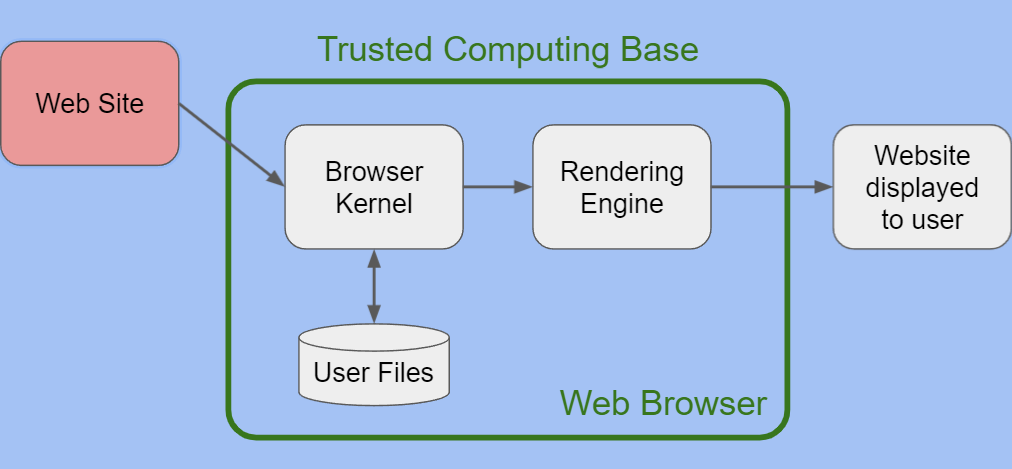
\includegraphics[scale=0.5]{assets/browser_design.png}
    \caption{Browser design.}
\end{figure}
\begin{figure}[!htb]
    \centering
    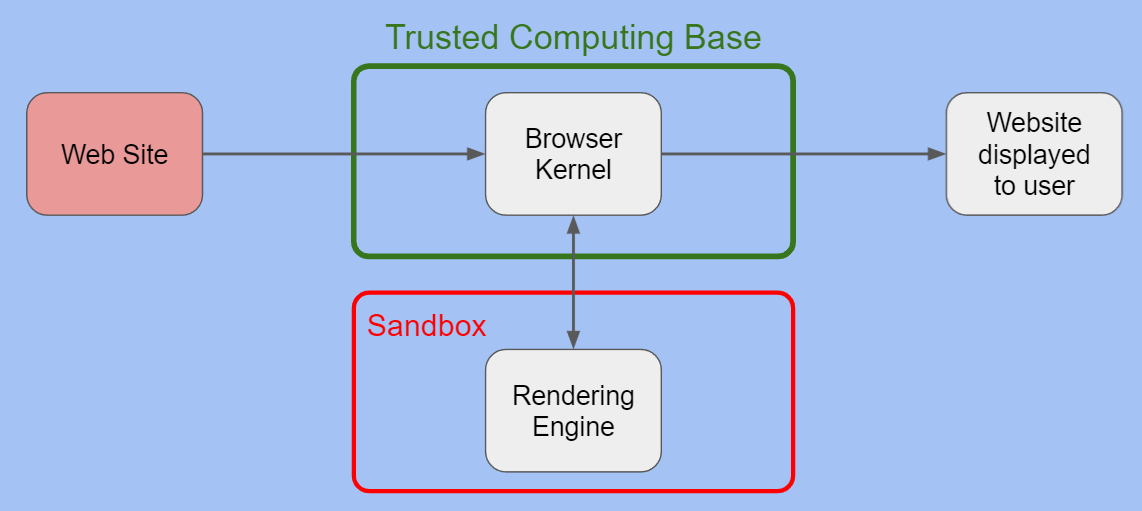
\includegraphics[scale=0.5]{assets/chrome_browser.png}
    \caption{Chrome Browser design.}
\end{figure}
\begin{example}
    Web Browser is an example of OS\newline
    Drive-by malware: malicious web page expolitsd browser bug to infect local files. \newline 
    The rendering engine is the part that interpreting programs so all the bugs live in rendering engine. So Chrome browser puts rendering engine into its own process. Goal: prevent "drive-by malware", where a malicious web page exploits a browser bug to infect local files. Now it sandboxes each web context so you can't even read out other web page content(E.g. spectre).
\end{example}
\textbf{Ensuring Complete Mediation}\newline
To secure access to some capability/resource, construct a reference monitor. Single point through which all access must occur(E.g. a network firewall). \newline Desired properties:
\itemnum
    \ii Un-bypassable("complete mediation")
    \ii Tamper-proof(is itself secure)
    \ii Verifiable(correct)
    \ii (Note, just restatements of what we want for TCBs)
\itemend
\textbf{Time of Check to TIme of Use, Vulnerability: Race Condition}\newline
procedure withdrawl(w)
\begin{enumerate}
    \ii let b := balance
    \ii if b $<$ w, abort
    \ii set bbalance := b - w
    \ii dispense \$w to user.
\end{enumerate}
Suppose that after step 2 here an attacker arranges to suspend first call, and calls withdrawl again concurrently.\newline
TOCTTOU=Time of Check to Time of Use.\newline
Ethereum is a cryptocurrency which offers "smart" contracts. The DAO(Distributed Autonomous Organization was an attempt to make a distributed mutual fund in Ethereum). Participants could vote on investments that should be made. The DAO supported withdrawals as well. To withdraw, the code was check the balance, then send the money, then decrement the balance. But sending money in Ethereum can send to another program written by the recipient. So someone "invested" then did a withdraw to this program which would initiate another withdraw.\newline 
\textbf{Separation of responsibility}
Example: Cinema, two-man rule in nuclear bunker.
\subsection{Summary}
\textbf{Notions Regarding Managing Privilege}:\newline
\itemnum
    \ii Least privilege: The notion of avoiding having unnecessary privileges.
    \ii Privilege separation: A way to achieve least privilege by isolating access to privileges to a small Trusted Computing Base(TCB)
    \ii Separation of responsibility: If you need to have a privilege, consider requiring multiple parties to work together(collude) to exercise it
\itemend
\textbf{Dealing with Users}\newline
\itemnum
    \ii Psycholofical acceptability: Will users abide a security mechanism, or decide to subvert it?
    \ii Consider human factors: Does a security mechanism assume something abouyt human behavior when interacting with the system that might not hold, even in the absence of conscious decisions by the uses to subvert
\itemend
Ouvrage Schoenenbourg. Only as secure as the weakest link. A door lock is only as strong as the window.\newline
Don't rely on \textbf{security through obscurity}. Security through obscurity (STO) is a process of implementing security within a system by enforcing secrecy and confidentiality of the system's internal design architecture. Security through obscurity aims to secure a system by deliberately hiding or concealing its security flaws. Obscurity does help but you need to design you system so that it fails. Kerckhoffs's Principle: A cryptosystem should be secure even if everything about the system, except the key, is public knowledge. Shannon's Maxim: The enemy knows the system.\newline
\textbf{Trusted path}. Users need to know they are talking with legit system. System needs to know its talking with the legit user. These channels need to be unspoofable and private. ATM skimmers are a failure of the trusted path.\newline
\textbf{"Use fail-safe defaults."} But it can often be hard to determine. Default for access here is reasonable. Deny all except for an allowed user list. But when the power goes out. Should the lock fail shut/open?\newline
\textbf{Common Assumptions When Discussing Attacks} Attackers can interact with our systems \textbf{without particular noise}. Probing(poking at systems) may go unnoticed even if highly repetitive, leading to crashes, and easy to detect. It’s easy for attackers to know general information about their targets, OS types, software versions, usernames, server ports, IP addresses, usual patterns of activity, administrative procedures. Attackers can obtain access to a copy of a given system to measure and/or determine how it work. Attackers can make energetic use of automation, they can often find clever ways to automate. Attackers can pull off complicated coordination across a bunch of different elements/systems. Attackers can bring large resources to bear if req’d, computation, network capacity, but they are not super-powerful. If it helps the attacker in some way, \textbf{assume they can obtain privileges} But if the privilege gives everything away (attack becomes trivial), then we care about unprivileged attacks. The ability to robustly detect that an attack has occurred \textbf{does not replace desirability of preventing}. Infrastructure machines/systems are well protected (hard to directly take over). So a vulnerability that requires infrastructure compromise is less worrisome than same vulnerability that doesn’t. Network routing is hard to alter … other than with physical access near clients (e.g., “wifi/coffeeshop”). Such access helps fool clients to send to wrong place. Can enable Man-in-the-Middle (MITM) attacks. We worry about attackers who are lucky. Since often automation/repetition can help “make luck”: If its 1 in a million, just try a million times! Just because a system does not have apparent value, \textbf{it may still be a targe}. Attackers are mostly undaunted by fear of getting caught.
\section{Appendix}
\renewcommand{\listtheoremname}{List of Definitions and Theorems}
\listoftheorems[ignoreall,show={theorem,definition}]

\listoftodos

\end{document}